
\section{Logical layer}
This layer represents the pure software component of the system.\\
This layer handles the input of the messages to be transmitted, the communication and encoding to the control layer, and most importantly the decoding, interpretation and forwarding of the message to its final consumer.
Logical encoding may be able to add robustness to the unreliable aspects of the communication.
A good logical layer could handle bit recovery in cases where symbols are missing or mistaken, and overall reduction of noise importance. 
Also a basic communication protocol could help in making the communication more stable and structured.
The logical layer for the transmitter is not very complex, it takes some message as input, manipulates it to meet the encoding and protocol requirements and redirects it to the control layer in a certain way, as previously discussed. 
The focus of this section will therefore be shifted to the receiving side of the communication.
 
\begin{figure}[htbp] %  figure placement: here, top, bottom, or page
   \centering
   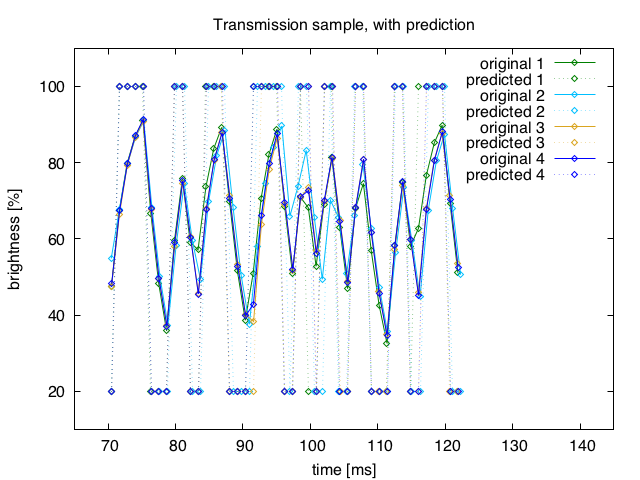
\includegraphics[height=200px]{img/sample} 
   \caption{Example of the results of interpreting digital information from analog input.}
   \label{fig:sample}
\end{figure}

%reading 
 \subsection{Reading the signal}
A key part of this layer is to convert analog sensor data representing light variations into binary code.
Fig. \ref{fig:sample} shows a sample of transmission. The green line represents the original values from the light sensor, while the purple line is a reconstruction of what the digital transmission would look like. 
Manchester encoding allows transmission to only have two kinds of peaks, either representing single bits, like a 1 or a 0, or two bits of the same kind, like a 11 or a 00.
This is because each binary 1 is represented as the sequence 01, and each 0 as 10.
Whenever two subsequent bits are different, there will be a sequence of two symbols of the same kind in Manchester encoding.
As an example, the sequence 0 0 0 0 0 0 0 1, representing the byte 1, would be encoded as 10 10 10 10 10 10 10 01.
When there is the switch between the binary 0 and the final bit 1, a sequence of two 0 symbols appear in the Manchester encoded byte.
During transmission this would translate to a longer and deeper 0 symbol, and it would be the same in reverse for a double 1.
Luckily, longer same symbol sequences are not possible with this encoding.\\

The design of an algorithm that could go through this sequences of sensory values and interpret them into binary data has undergone through different stages and different attempts.
\subsubsection{Machine Learning approach}
The first version of it made use of Machine Learning techniques to train a model with training data, "teaching" a classifier what kinds of data and results one would expect in this application. The data was taken in different circumstances of ambient light interference, with different messages sent and at different times.
Multiple classifiers were tested, with a maximum success rate of about 75\% of correct predictions. The classifiers included NaiveBayes, RandomForest, AdaBoost and ArtificialNeuralNetworks, all with comparable results.\\
There were major difficulties with this approach. For starters, there were problems identifying the labels to train these models, namely the classes or categories where the data would belong.
Initially, the four categories were "1", "0", "11", and "00". The basic idea is that given a sequence of values it should fall in one of these four classes.
The problem was though that single bits and double bits have different sizes in amount of values that are received from the sensor. This size is also called the number of features.\\
Most standard modules for machine learning require the same number of features for all the labels.\\
In order to get around this rule, the labels became "10", "01", "11", and "00". Eventually, also these labels were produced by different numbers of features. Other combinations were tried, and eventually all leading to the same result. 
One way to get around this problem was to have a fixed number of features, but big enough to include all the possibilities. Samples smaller than this maximum amount (virtually all of the samples) would be filled up with blank values until they reached the intended size.\\
Another way would be to train a classifier for each specific number of features that may occur. In this case, the amount of classifiers needed would be around 4, for number of features ranging between 7 and 10.
The downside of this approach is that each classifier becomes very specific to a restricted set of the training data, potentially loosing track completely of certain labels.\\
The final setup for machine learning prediction used the labels "101", "100", "011", "110", "001", "11", "00", "10", "01", scaling of the features and larger sample size to be filled up with blanks. This produced overall the best results for the machine learning approach, but never above 80\% success rate.\\
A second downside to this approach would be that when receiving values from the sensor in real time, one would need to keep a moving window  of the size of the number of features and try to obtain a prediction from the classifier each time.
This might likely slow down the reading process.\\

\subsubsection{Custom algorithm approach}
These poor results ultimately led to a change of approach for reading the data. 
Just looking at fig. \ref{sample} it's pretty straightforward to see that the high peaks represent 1s and the low peaks represent 0s. 
By setting some rules, a custom classifier could predict a result without the need to be trained with sample data.
In particular, the classifier analyses sequences of values, trying to find sequences that are either monotonically increasing or monotonically decreasing.
Also a noise factor has to be taken into account, in this way small enough variations are not considered.
As mentioned before, there are only two kinds of peaks in the sequences, either single or double peaks.
Therefore, it's of critical importance to be able to distinguish the two cases. One criteria that was originally deployed for this was to count the number of values that progress in the same direction, either up or down. 
This was later changed to the more precise criteria of duration of such sequences, and for this reason for each sensor value a timestamp is also included in the control layer, representing the time of reception for that specific value.\\ 
With this in mind, the algorithm has been developed to very simply count the duration of either monotonically increasing or decreasing sequences of values, and produce a prediction when the direction changes, based on such duration.
This technique performs particularly well in this application, producing up to 100\% success rate in certain cases.
 Runtime wise, the algorithm takes constant time for each value that is received, and may or may not produce a resulting prediction.
A simplified version of the algorithm can be found in fig. \ref{code}, written in Python 2.7.
The algorithm has been simplified to be more readable.

\subsection{Protocol}
As can be seen the rates of transmission and reception in this prototype system are not very high, if compared to average wireless transmission speeds, which are measured in Mbps.
Transmission in visible light is also exposed to a high degree of uncertainty, depending on parameters like distance, maximum brightness, interference, noise, and so on.
In this prototype, communication is only established in one direction, which additionally increases the threat of getting wrong results.
In order to compensate all this aspects, an effort to strengthen the success rate has been made by structuring the communication into a very basic protocol.
Each PDU is included between two single bytes: STX, that indicates the start of a message, and a byte ETX which indicates its end. These two are bytes 0x02 and 0x03 respectively. To avoid that the reader assumes an ETX byte wrongfully while reading the message, a length byte LEN is also included in the header of the PDU, to specify the length of the message in bytes.
Additionally, each PDU is restrained to have a maximum size, and longer messages need to be split into more PDUs.
This is mostly to preserve the serial connection between logical layer and control layer to overflow the serial buffer.
This three fields combined should make it fairly easy for the receiver to know if some parts of the message were lost during transmission.
Since the communication is established mono directionally, the transmitter wouldn't know if the message was delivered, but the receiver most likely would.
Mistaken symbols are very unlikely in this kind of communication, it is much more likely to entirely miss some.
Therefore the receiver could easily know if the message was delivered or not.
To increase reliability, the transmitter could be transmitting the same message over and over.

\subsubsection{Additional fields}
Increasing the functionalities or complexity of the system, additional parameters in the PDU might result useful if not necessary. 
Imagining a scenario with multiple receivers of messages broadcasted through light in a unilateral way, a receiver field could be added to the PDU. Also, it would be wise to perform encryption on the PDUs, in a way that only the intended receivers would be able to read the message directed to them.
Establishing 2-way communication would also require more steps. 2-way communication would be a very good way to ensure correctness of the transmission. For this, at least 2 more parameters seem necessary: a sequence number to identify the packet, and a checksum to check correctness of the received message.
A header for visible light communication doesn't require many parameters since it's likely to be the very last end of a communication process. Since it's mainly short distanced, it doesn't need any routing parameters as it would in big networks. 

\begin{figure}
\centering
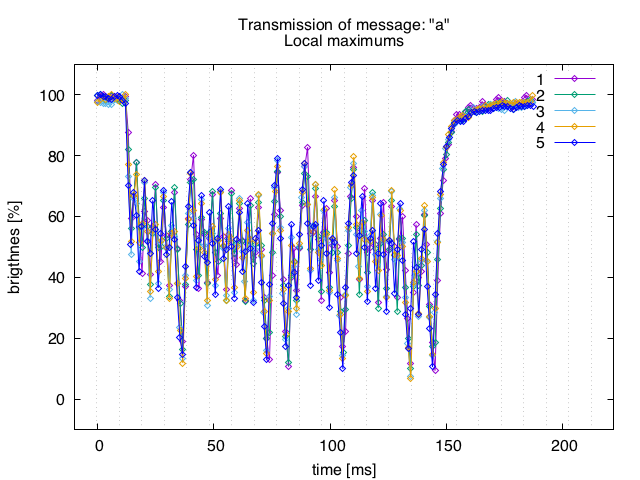
\includegraphics[height=180px]{img/transmission}
\caption{Example of transmission of message "a", the transmission include STX, ETX, and LEN bytes.}
\label{fig:transmissionA}
\end{figure}

\subsection{Results}
 \todo{protocol vs no protocol? bits correct per bits sent? compare other technologies?}

Figure \ref{fig:transmissionA} shows an example of the transmission of the message "a", including STX, ETX and LEN bytes.
In ASCII, letter "a" is represented by the byte 97, or 01100001 in binary.
As previously mentioned, the STX is byte 2, ETX byte 3, and LEN in this case would be 1.
In binary, the entire message would then be: 00000010 - 00000001 - 01100001 - 00000011.
In Manchester encoding: 1010101010100110 - 1010101010101001 - 1001011010101001 - 1010101010100101.
The traits of the signal in the figure can be visibly associated with the Manchester encoding of the message, clearly visible at least in the occurrence of double symbols. 
A 00 and a 11 are clearly visible at the end of the first byte, a 00 almost conclude the second byte, follows a 11 connecting the second to the third byte, then a 00, 11, and so on.

\subsubsection{Experimental setup}
To test performance of the communication at its final stage, multiple tests have been performed on the prototype.
For each test, the system takes user input for initialising the message to send, encodes it and sends it through light. 
The receiver reconstructs the message depending on values retrieved from the sensor.
Tests have been performed at very close proximity of the sensor to the light source, without other lights directly facing the sensor but with presence of natural light.
A test is considered successful if every bit is correctly received and interpreted.
Messages of different sizes have been tested.
Table \ref{tab:txresults} illustrates the results of these tests.

\begin{table}[hbt]
\centering
  \begin{tabular}{l c c c}
    distance & ambient light & tests & successful \\
    \hline
   0 cm & yes & 50 & 100\% \\
   0 cm & yes & 50 & 100\% \\
   0 cm & yes & 50 & 100\% \\
   0 cm & yes & 50 & 100\% \\
   10 cm & yes & 50 & 92\% \\
   10 cm & yes & 50 & 96\% \\
   10 cm & yes & 50 & 88\% \\
   10 cm & yes & 50 & 60\% \\
  \end{tabular}
  \caption{Tests of full transmission, success criteria is 100\% correctness.}
  \label{tab:txresults}
\end{table}


\begin{figure}
\centering
\begin{lstlisting}[language=Python, frame={}]
	def feed(self, time, value):
		pred = None
		
		# staying
		if abs(value - self.prev) <= self.epsilon:
			pass

		#going down
		elif value <= self.prev: 
			if self.direction: # up	
				pred = self._predict(time)

		# going up
		elif value > self.prev: 
			if not self.direction: # down
				pred = self._predict(time)

		self.prev = value
		return pred
		
	def _predict(self, time):
		m = self.direction
		delta = time - self.seqstart
		pred = '-'
		
		if delta >= self._doubletime:
			pred = '11' if m else '00'
		else:
			pred = '1' if m else '0'

		self.direction = not self.direction
		self.seqstart = time
		return pred
\end{lstlisting}
\caption{Simplified algorithm for signal interpretation (Python 2.7).}
\label{code}
\end{figure}